\documentclass[12pt,letterpaper]{article}
\usepackage{fullpage}
\usepackage[top=2cm, bottom=4.5cm, left=2.5cm, right=2.5cm]{geometry}
\usepackage{amsmath,amsthm,amsfonts,amssymb,amscd}
\usepackage{lastpage}
\usepackage{enumerate}
\usepackage{fancyhdr}
\usepackage{mathrsfs}
\usepackage{xcolor}
\usepackage{fancyvrb}
\usepackage{graphicx}
\usepackage{listings}
\usepackage{hyperref}
\usepackage{tikz}
\usepackage{relsize}
\usepackage{fancyvrb}
\usepackage{import}
\usetikzlibrary{shapes.geometric,fit}

\hypersetup{%
  colorlinks=true,
  linkcolor=blue,
  linkbordercolor={0 0 1}
}

\setlength{\parindent}{0.0in}
\setlength{\parskip}{0.05in}

\theoremstyle{definition}
\newtheorem*{statement}{Statement}
\newtheorem*{claim}{Claim}
\newtheorem*{theorem}{Theorem}
\newtheorem*{lemma}{Lemma}

\newcommand{\contra}{\Rightarrow\!\Leftarrow}
\newcommand{\R}{\mathbb{R}}
\newcommand{\F}{\mathbb{F}}
\newcommand{\Z}{\mathbb{Z}}
\newcommand{\Zeq}{\mathbb{Z}_{\geq 0}}
\newcommand{\Zg}{\mathbb{Z}_{>0}}
\newcommand{\Req}{\mathbb{R}_{\geq 0}}
\newcommand{\Rg}{\mathbb{R}_{>0}}
\newcommand{\N}{\mathbb{N}}
\newcommand{\Q}{\mathbb{Q}}
\newcommand{\C}{\mathbb{C}}
\DeclareMathOperator{\Cov}{Cov}
\DeclareMathOperator{\Var}{Var}

\newcommand{\incfig}[1] {%
    % \def\svgwidth{\columnwidth}
    \import{./figures/}{#1.pdf_tex}
}

\title{ECON 3412 HW 2}
\author{David Chen, dc3451}

\begin{document}

\maketitle
% \today

\section*{Problem 1}

The \verb|R| code to generate the following output can be found in problem 2.

\begin{Verbatim}[fontsize=\small]
a)
         country cigarettes covid
1  United States     1016.6 320.0
2         France     1089.9 448.4
3 United Kingdom      827.7 575.4
4         Canada     1021.3 219.5
5          Italy     1493.3 561.3
6        Germany      720.1 195.7
b) Sample mean of X:  1028.15
b) Sample mean of Y:  386.7167
b) Sample standard deviation of X:  266.6207
b) Sample standard deviation of Y:  166.6046
c) Correlation coefficient between X, Y:  0.4860556
d) The OLS regression is given by the following:


Call:
lm(formula = Y ~ X, data = problem1)

Residuals:
      1       2       3       4       5       6
 -63.21   42.93  249.56 -165.14   33.31  -97.45

Coefficients:
            Estimate Std. Error t value Pr(>|t|)
(Intercept)  74.4428   288.4930   0.258    0.809
X             0.3037     0.2730   1.112    0.328

Residual standard error: 162.8 on 4 degrees of freedom
Multiple R-squared:  0.2363,	Adjusted R-squared:  0.04531
F-statistic: 1.237 on 1 and 4 DF,  p-value: 0.3283

d) Estimated intercept term beta_0:  74.44284
d) Estimated slope coefficient beta_1:  0.303724
e) The equation of the regression is then Y_hat = 74.44284 + 0.303724 X
f) We have that the estimated Y_i are
         country cigarettes predicted.covid.Y_i
1  United States     1016.6            383.2087
2         France     1089.9            405.4716
3 United Kingdom      827.7            325.8352
4         Canada     1021.3            384.6362
5          Italy     1493.3            527.9939
6        Germany      720.1            293.1545
g) The OLS residuals are
         country cigarettes predicted.residuals.u_i
1  United States     1016.6               -63.20865
2         France     1089.9                42.92838
3 United Kingdom      827.7               249.56481
4         Canada     1021.3              -165.13616
5          Italy     1493.3                33.30612
6        Germany      720.1               -97.45449
\end{Verbatim}

\section*{Problem 2}
\subsection*{a}
The following \verb|R| code plots the scatterplot and OLS line:
\begin{Verbatim}[fontsize=\small]
ggplot(problem1, aes(X, Y)) + geom_point() + xlim(0,1600) + geom_smooth(method = "lm") +
  xlab("Cigarettes consumed per capita in 2019") +
  ylab("COVID-19 deaths per million people by Match 31 2020")
\end{Verbatim}
which looks like this:
\begin{center}
  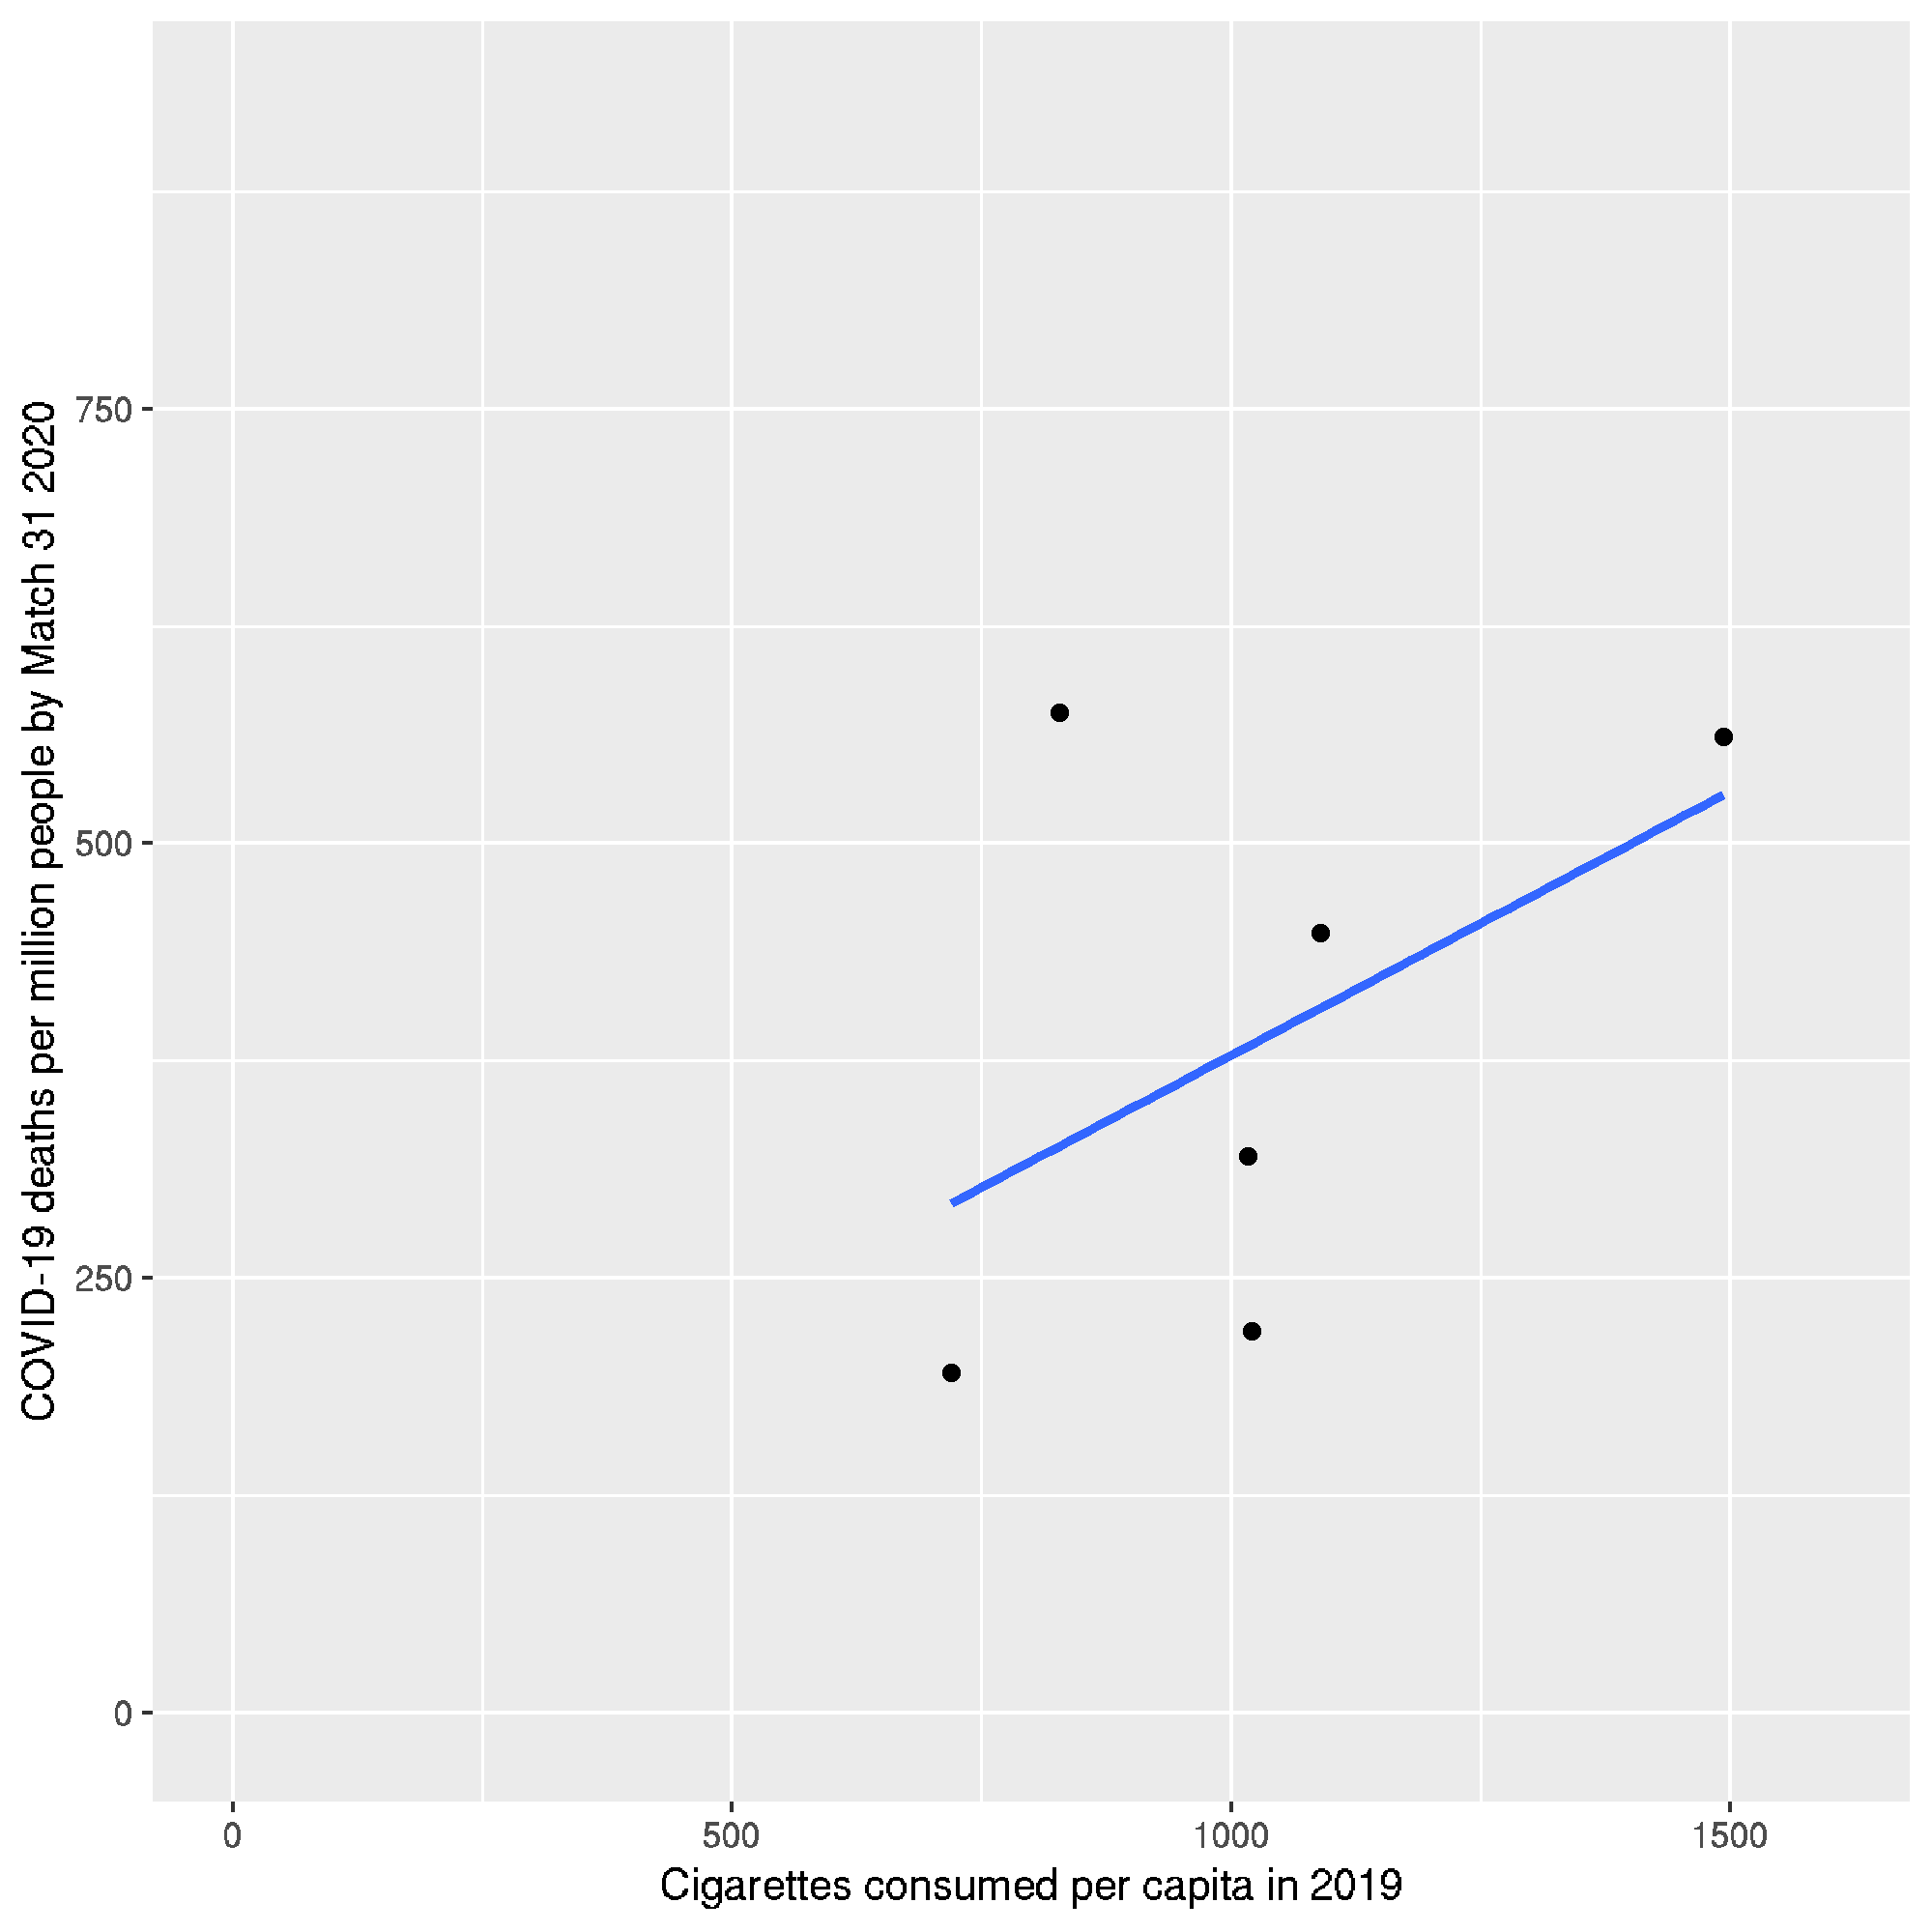
\includegraphics[width=13cm]{./problem2.png}
\end{center}

\subsection*{b}

% TODO

The sample intercept of \(74.44\) implies that \(74.44\) COVID-19 deaths per million people is the amount of deaths per million that a country that does not smoke at all will suffer, on average.

The sample slope of \(0.304\) implies that for every unit increase in cigarettes consumed per capita in 2019, we would, according to the model, see an increase of \(0.304\) deaths per million people due to COVID on average in a country.

The actual amount of inference we can do is probably small; we have small sample sizes and probably have omitted variable bias; for example, the amount of cigarettes consumed per capita is probably correlated with the efficacy of public health policy in a given country, which probably determines also the efficacy of said country's COVID response.

\subsection*{c}

\begin{Verbatim}[fontsize=\small]
problem1 <- read.csv("problem1.csv")
X <- problem1$cigarettes
Y <- problem1$covid
ols <- lm(Y ~ X, data = problem1)
summ <- summary(ols)
beta_0 <- summ$coefficients[1]
beta_1 <- summ$coefficients[2]

message("a)")
print(problem1)
cat("b) Sample mean of X: ", mean(X), "\n")
cat("b) Sample mean of Y: ", mean(Y), "\n")
cat("b) Sample standard deviation of X: ", sqrt(var(X)), "\n")
cat("b) Sample standard deviation of Y: ", sqrt(var(Y)), "\n")
cat("c) Correlation coefficient between X, Y: ", cor(X, Y), "\n")
message("d) The OLS regression is given by the following:\n")
print(summ)
cat("d) Estimated intercept term beta_0: ", beta_0, "\n")
cat("d) Estimated slope coefficient beta_1: ", beta_1, "\n")
cat("e) The equation of the regression is then Y_hat =",
    beta_0, "+", beta_1, "X\n")
cat("f) We have that the estimated Y_i are\n")
print(data.frame("country"=problem1$country,
                 "cigarettes"=problem1$cigarettes,
                 "predicted covid Y_i"=predict(ols)))
cat("g) The OLS residuals are\n")
print(data.frame("country"=problem1$country,
                 "cigarettes"=problem1$cigarettes,
                 "predicted residuals u_i"=ols$residuals))
\end{Verbatim}

\verb|problem1.csv| contains the following:
\begin{Verbatim}[fontsize=\small]
country,cigarettes,covid
United States,1016.6,320
France,1089.9,448.4
United Kingdom,827.7,575.4
Canada,1021.3,219.5
Italy,1493.3,561.3
Germany,720.1,195.7
\end{Verbatim}


\section*{Problem 3}
\subsection*{a}

There are a multitude of omitted factors that can be contained in $u$; after all, it would be highly shocking if education was the sole determiner of the amount of children a woman has. We can come up with a few easy examples of omitted factors:
\begin{enumerate}
  \item Income/Wealth: it's generally well known that richer countries have a lower fertility rate than poorer ones. One would expect this relationship to hold true on an individual basis as well, due to factors such as poorer access to birth control or sexual education. In particular, the latter is a consequence of education and income being positively correlated, so this probably implies some omitted variable bias in the naive regression.
  \item Religious Affiliation: for example, it's somewhat well known that Catholics tend to have more children than non-Catholics. The correlation with education is a little unclear here, though: Christians are actually more likely, for instance, in the US to be college educated than non-Christians, but this trend doesn't hold true for non-Christian religions in the US.
  \item Race/Ethnicity: for example, it's generally well known that for whatever reason, Asian immigrants in the US tend to have less children than other races. The correlation with education is present: Asian people are more likely to be college educated than white people, who in turn are more likely to be college educated than black people.
  \item Age: older women probably have more children than younger women, if only for the fact that someone who is 55 has had more chances to have a child than someone who is 25. You would also expect some correlation with education, with younger women having more access to education given historical discrimination in higher education.
\end{enumerate}

\subsection*{b}

The presence of factors which will have some impact on the amount of kids that a woman has that are also correlated with years of education implies that omitted variable bias will be present. For example, let us take the first example of omitted income. We expect that \(\hat{b}\) is overestimated in a simple regression, as we have that \(\hat{b} \rightarrow b + c\rho\) (in probability), where \(c\) is a positive constant given by the ratio of standard deviations of income and education, and \(\rho\) is the correlation between income and education; in particular, we expect that wealthier people will go to college more often on average, so \(\rho > 0\), and so \(\hat{b} > b\), and the effect of education is overstated.

This means that we cannot find the ceteris paribus effect of education on fertility this way.

\section*{Problem 4}

\subsection*{a}

Note that \(MALE = 0\) gives \(WAGE = 12.68\) as the average \$/hour earnings of females; similarly, \(MALE=1\) gives that \(WAGE = 15.47\) is the average \$/hour earnings of males. This implies that \(15.47 - 12.68 = 2.79\), the coefficient of \(MALE\) is the estimated wage gap. The ``slope'' is to be interpreted here as the estimated difference between population means.

\subsection*{b}

The corresponding \(t\)-statistic for \(\beta_{1}\)is \(\frac{\hat{\beta_{1}} - \beta_{1,0}}{SE(\hat{\beta_{1}})} = \frac{2.79}{0.84} = 3.32\). In a two sided test that \(\beta_{1} \neq 0\) we have that (we just use the normal distribution here, since \(n\) is large) the \(p\)-value is \(2(1-\Phi(3.32)) = 0.0009\). If we want a one-sided test that \(\beta_{1} > 0\), the corresponding \(p\)-value is \(1 - \Phi(3.32) = 0.00045\).

\subsection*{c}

Same as part a: \(MALE = 0\) gives \(WAGE = 12.68\) as the average \$/hour earnings of females; similarly, \(MALE=1\) gives that \(WAGE = 15.47\) is the average \$/hour earnings of males.

\subsection*{d}

Keeping in mind the semantic meanings of the coefficients, we would need that the intercept be the average \$/hour earnings of males, and the slope the negative of the current slope (as the order of subtraction is reverse). Thus, we would get a regression of
\[
  WAGE = 15.47 - 2.79 \times FEMALE
\]

The $R^{2}$ and standard errors do not change.

\section*{Problem 5}

Note: since I am using \verb|R|, there is no robust option, with OLS regression defaulting to homoskedasticity. There is a way to replicate STATA however, according to \href{https://stats.stackexchange.com/questions/117052/replicating-statas-robust-option-in-r/117066#117066}{this StackExchange post}, which is what I will be using.

\subsection*{a}

We get the following output
\begin{Verbatim}[fontsize=\small]
Nonrobust:

Call:
lm(formula = ahe ~ female)

Residuals:
    Min      1Q  Median      3Q     Max
-20.347  -8.090  -3.090   5.016  83.381

Coefficients:
            Estimate Std. Error t value Pr(>|t|)
(Intercept)  22.3879     0.1873 119.542   <2e-16 ***
female       -2.7598     0.2901  -9.515   <2e-16 ***
---
Signif. codes:  0 ‘***’ 0.001 ‘**’ 0.01 ‘*’ 0.05 ‘.’ 0.1 ‘ ’ 1

Residual standard error: 12.05 on 7096 degrees of freedom
Multiple R-squared:  0.0126,	Adjusted R-squared:  0.01246
F-statistic: 90.53 on 1 and 7096 DF,  p-value: < 2.2e-16

Robust:

t test of coefficients:

            Estimate Std. Error  t value  Pr(>|t|)
(Intercept) 22.38794    0.20088 111.4476 < 2.2e-16 ***
female      -2.75982    0.28122  -9.8137 < 2.2e-16 ***
---
Signif. codes:  0 ‘***’ 0.001 ‘**’ 0.01 ‘*’ 0.05 ‘.’ 0.1 ‘ ’ 1
\end{Verbatim}

The addition of heteroskedastic standard errors does affect the significance of the \(t\)-test, with \(p\)-values in the \(10^{-16}\) range in either case; we have very strong evidence that there is a statistically meaningful gender wage gap in the context of this model. In particular, the coefficient of \(-2.75982\) means that women on average make \(\$2.76\) less per hour than men.

In particular, we surprisingly get a smaller standard error for the coefficient of female (the actual estimators are unchanged, as we would expect), but we do see a larger standard error for the intercept.

\subsection*{b}

We get the following graph from this \verb|R| code:

\begin{Verbatim}[fontsize=\small]
ggplot(nonrobust_ols, aes(female, ahe)) + geom_point() + geom_smooth(method = "lm") +
xlab("female (1 = female, 0 otherwise)") + ylab("Average Hourly Earnings")
\end{Verbatim}

\begin{center}
  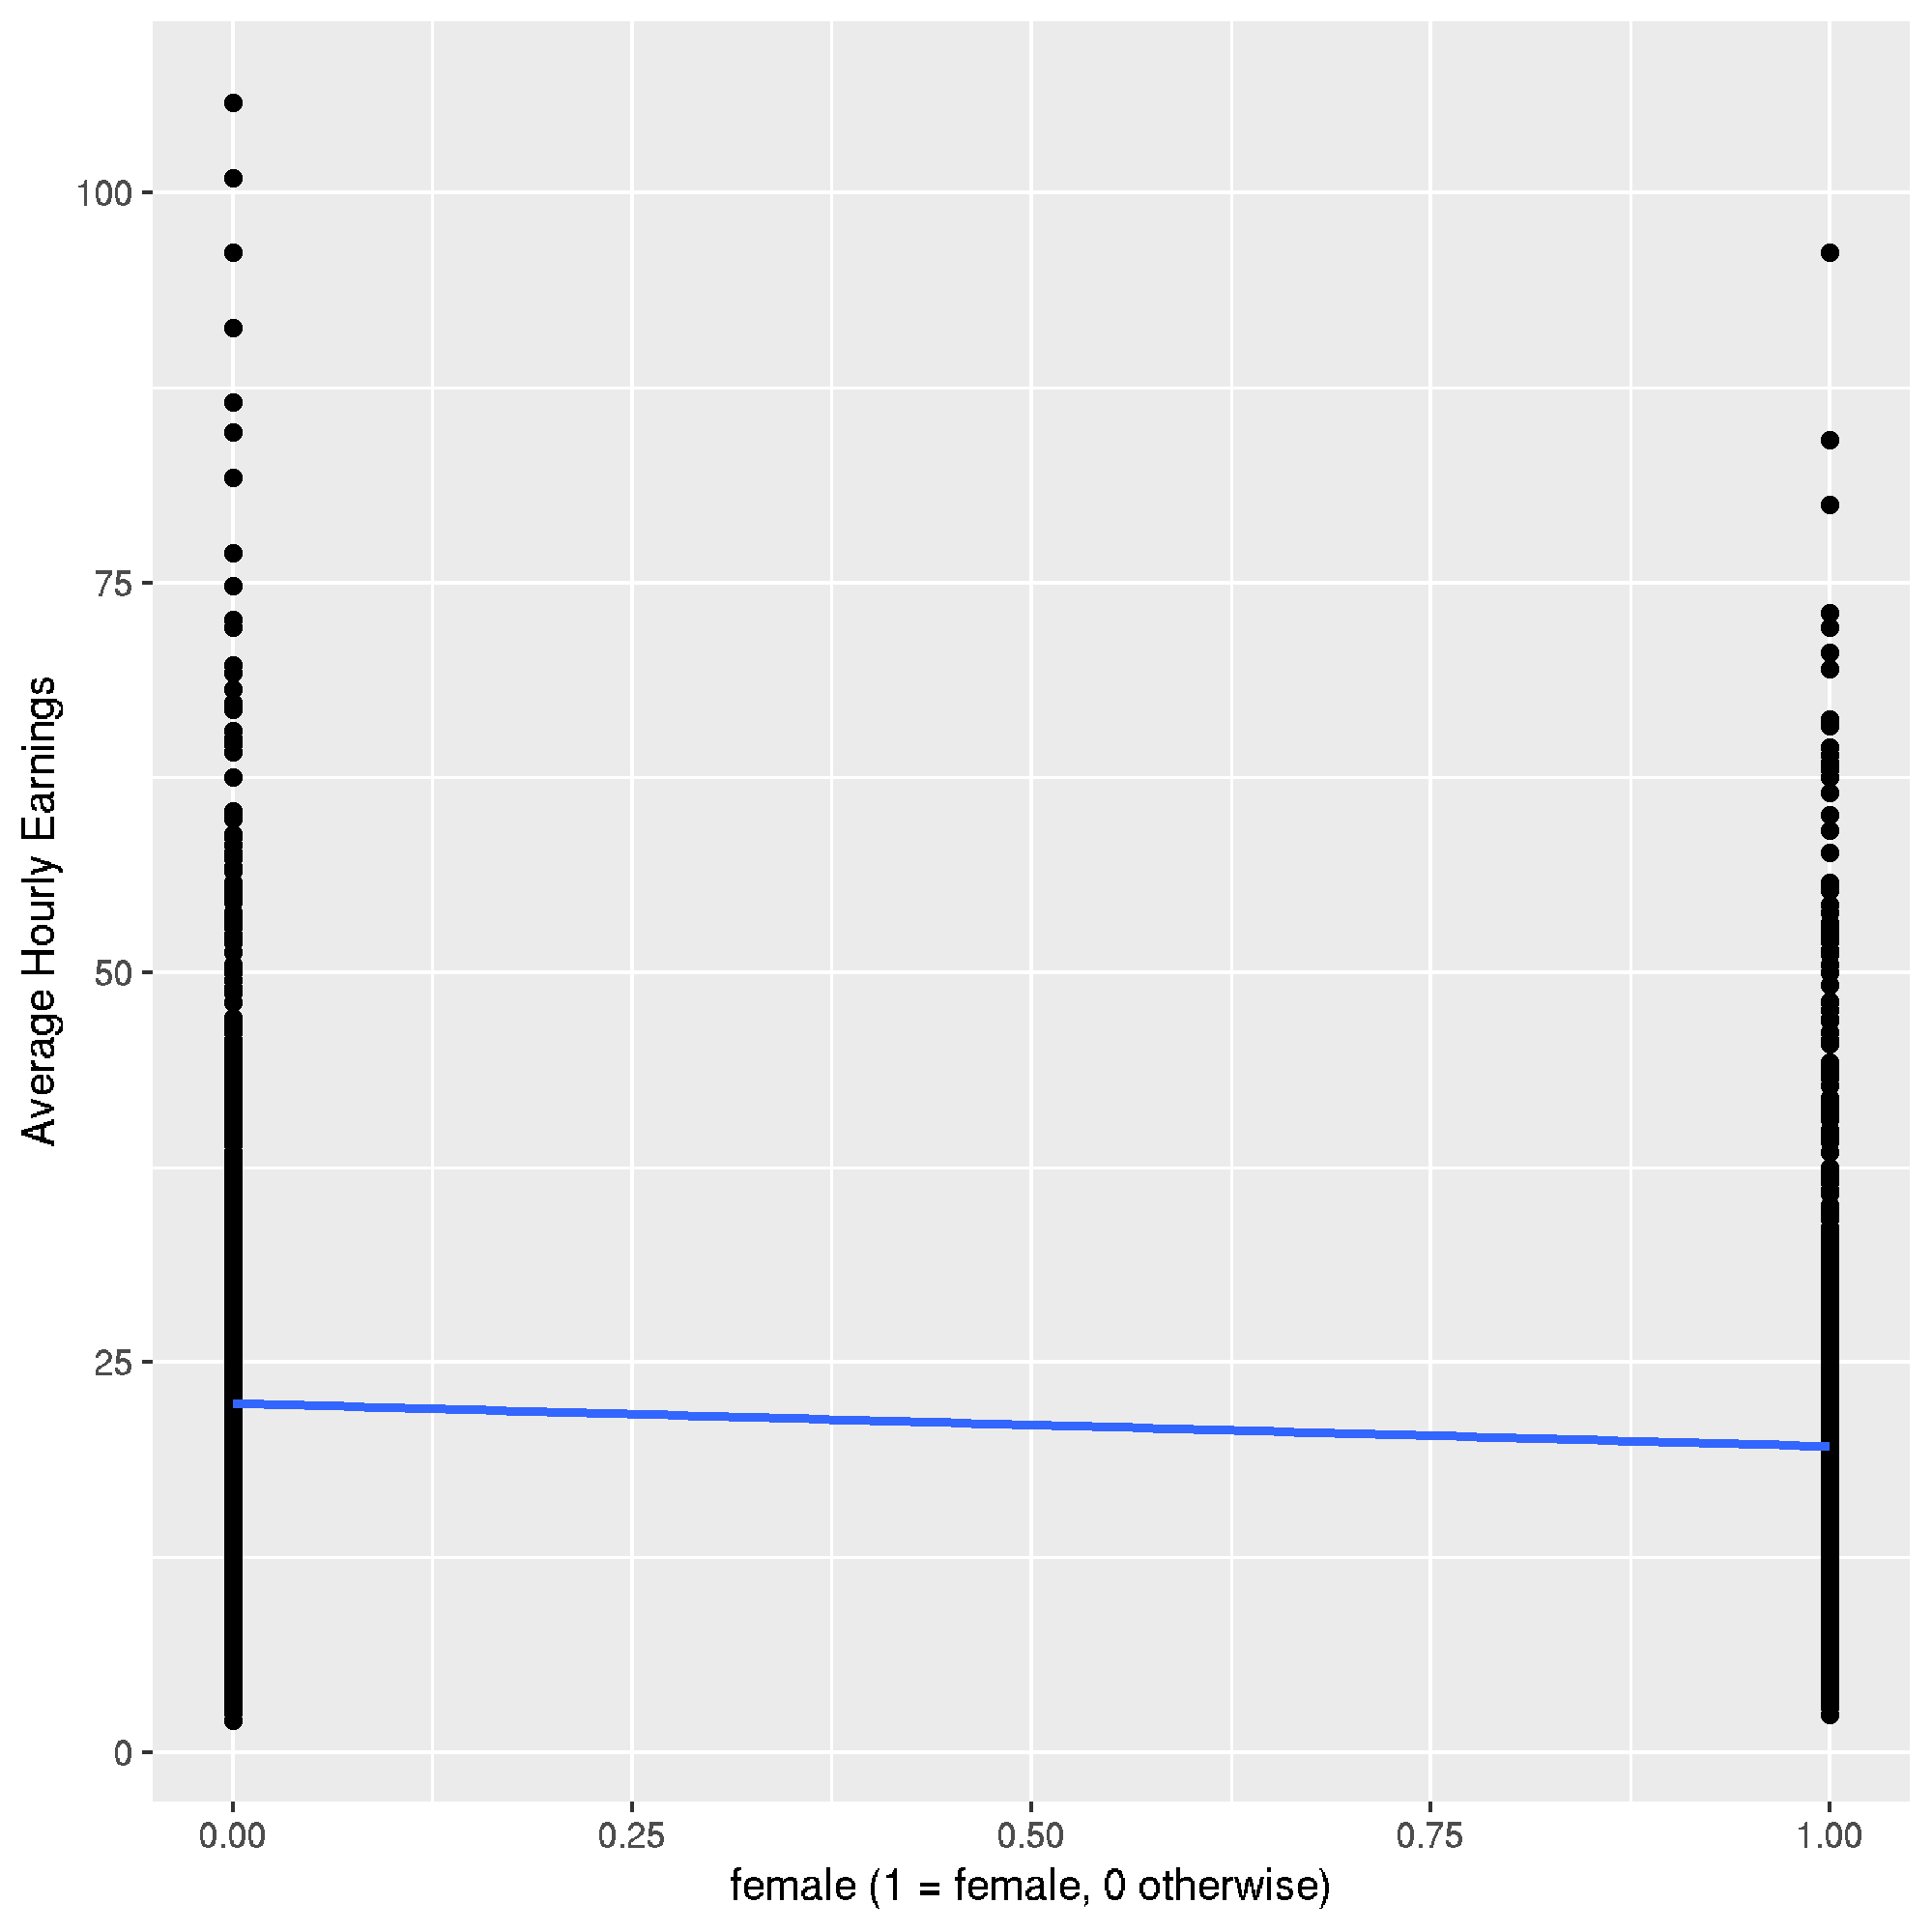
\includegraphics[width=13cm]{./problem5.png}
\end{center}

This does suggest some amount of heteroskedasticity, as we see that the incomes for men have a fatter right tail, i.e. there are more men who make far more than the male average than there are women who make far more than the female average, suggesting that the variance of $u \mid female = 0$ is larger than $u \mid female = 1$.

\subsection*{c}

The critical value for \(99\%\) intervals in this case is \(\Phi^{-1}(0.995) = 2.575\), so the corresponding \(99\%\) CI with the robust standard error of \(0.281\) is \(-2.7598 \pm 2.575(0.28122) = (-3.48529, -2.0343)\).

\subsection*{d}

We have the following:
\begin{Verbatim}[fontsize=\small]
Nonrobust with age:

Call:
lm(formula = ahe ~ female + age)

Residuals:
    Min      1Q  Median      3Q     Max
-22.654  -8.125  -2.775   5.135  82.687

Coefficients:
            Estimate Std. Error t value Pr(>|t|)
(Intercept)  6.42164    1.47736   4.347  1.4e-05 ***
female      -2.65998    0.28783  -9.241  < 2e-16 ***
age          0.53744    0.04933  10.894  < 2e-16 ***
---
Signif. codes:  0 ‘***’ 0.001 ‘**’ 0.01 ‘*’ 0.05 ‘.’ 0.1 ‘ ’ 1

Residual standard error: 11.95 on 7095 degrees of freedom
Multiple R-squared:  0.02884,	Adjusted R-squared:  0.02857
F-statistic: 105.4 on 2 and 7095 DF,  p-value: < 2.2e-16

Robust with age:

t test of coefficients:

            Estimate Std. Error t value  Pr(>|t|)
(Intercept)  6.42164    1.44260  4.4514  8.66e-06 ***
female      -2.65998    0.27926 -9.5250 < 2.2e-16 ***
age          0.53744    0.04885 11.0020 < 2.2e-16 ***
---
Signif. codes:  0 ‘***’ 0.001 ‘**’ 0.01 ‘*’ 0.05 ‘.’ 0.1 ‘ ’ 1
\end{Verbatim}

The coefficient of female did in fact change, but not by a lot (from \(-2.76\) to \(-2.66\)).

\subsection*{e}

The coefficient of age here is \(0.53744\), so we expect on average, someone who is older by one year than someone else of the same gender should make \(53\) cents more per hour than their counterpart.

\section*{Problem 6}
\subsection*{a}

\begin{align*}
  E[\hat{\beta}_{1}] &= \frac{\Cov(Earnings, Female_{i})}{\Var(Female_{i})} \\
                     &= \frac{\Cov(\beta_{0} + \beta_{1}Female_{i} + \beta_{2}Bachelors_{i} + u_{i}, Female_{i})}{\Var(Female_{i})} \\
                     &= \frac{\Cov(\beta_{1}Female_{i} + \beta_{2}Bachelors_{i} + u_{i}, Female_{i})}{\Var(Female_{i})} \\
                     &= \frac{\Cov(\beta_{1}Female_{i},Female_{i})}{\Var(Female_{i})} + \frac{\Cov(\beta_{2}Bachelors_{i},Female_{i})}{\Var(Female_{i})} + \frac{\Cov(u_{i},Female_{i})}{\Var(Female_{i})} \\
                     &= \beta_{1}\frac{\Cov(Female_{i}, Female_{i})}{\Var(Female_{i})} + \beta_{2}\frac{\Cov(Bachelors_{i},Female_{i})}{\Var(Female_{i})} + \frac{\Cov(u_{i},Female_{i})}{\Var(Female_{i})} \\
  \intertext{Since we have that \(\Cov(X,X) = \Var(X)\),}
                     &= \beta_{1} + \beta_{2}\frac{\Cov(Bachelors_{i},Female_{i})}{\Var(Female_{i})} + \frac{\Cov(u_{i},Female_{i})}{\Var(Female_{i})} \\
  \intertext{Since we have that \(E[u_{i} \mid Female_{i}] = 0\), as this is an OLS construction \textit{assumed} to be ``true'', we have from the last homework that \(\Cov(u_{i}, Female_{i}) = 0\), so}
                     &= \beta_{1} + \beta_{2}\frac{\Cov(Bachelors_{i},Female_{i})}{\Var(Female_{i})}
\end{align*}
so the omitted variable bias seems to be \(\beta_{2}\frac{\Cov(Bachelors_{i},Female_{i})}{\Var(Female_{i})}\).

\subsection*{b}

\begin{itemize}
  \item \(\beta_{1}\) ought to be negative; we would expect, given the history of gender-based discrimination, that female wages are lower on average than male wages, even accounting for education.
  \item \(\beta_{2}\) is probably positive: it is well known that college graduates make more money than non college graduates on average.
  \item \(\frac{\Cov(Bachelors_{i}, Female_{i})}{\Var(Female_{i})}\) has its sign determined entirely by \(\Cov(Bachelors_{i}, Female_{i})\), as the variance in the denominator is always positive. The sign of this covariance is actually unclear in the US. Recently, women have undergraduate degrees in the same proportion as men (or higher!), but this wasn't true, say a decade ago. It depends on age, really: older generations have more men with bachelors, but younger generations have more women with bachelors.

    In non-US countries, men probably are more likely to have a bachelors, so the covariance is negative.
\end{itemize}

In the case that the covariance is negative, then the omitted variable bias is negative (that is, $E[\hat{\beta}_{1}] < \beta_{1}$; however, since we expect \(\beta_{1} < 0\), this means that we are overestimating the magnitude of the effect of being female on wages). Similarly, if the covariance is positive, \(\hat{\beta}_{1} > \beta_{1}\) and we are underestimating the magnitude of the effect of being female on wages.

\subsection*{c}

We get the following:
\begin{Verbatim}[fontsize=\small]
Nonrobust with bachelors:

Call:
lm(formula = ahe ~ female + bachelor)

Residuals:
    Min      1Q  Median      3Q     Max
-25.639  -6.762  -2.040   4.342  82.575

Coefficients:
            Estimate Std. Error t value Pr(>|t|)
(Intercept)  17.8227     0.2107   84.57   <2e-16 ***
female       -4.2439     0.2683  -15.82   <2e-16 ***
bachelor      9.8569     0.2650   37.20   <2e-16 ***
---
Signif. codes:  0 ‘***’ 0.001 ‘**’ 0.01 ‘*’ 0.05 ‘.’ 0.1 ‘ ’ 1

Residual standard error: 11.02 on 7095 degrees of freedom
Multiple R-squared:  0.1738,	Adjusted R-squared:  0.1735
F-statistic: 746.1 on 2 and 7095 DF,  p-value: < 2.2e-16

Robust with bachelors:

t test of coefficients:

            Estimate Std. Error t value  Pr(>|t|)
(Intercept) 17.82266    0.17885  99.649 < 2.2e-16 ***
female      -4.24393    0.26473 -16.031 < 2.2e-16 ***
bachelor     9.85693    0.26376  37.370 < 2.2e-16 ***
---
Signif. codes:  0 ‘***’ 0.001 ‘**’ 0.01 ‘*’ 0.05 ‘.’ 0.1 ‘ ’ 1
\end{Verbatim}

This an estimate of \(\beta_{2}\) as \(9.857\); this can be interpreted as that within the same gender, on average, a person with a bachelor makes \(\$9.867\) more per hour than their non-college educated counterpart.

\subsection*{d}

This is reasonable: the desired covariance in the dataset can be computed to be

\verb|cov(cps_data$female, cps_data$bachelor) = 0.0366|

and the desired variance to be

\verb|var(cps_data$female) = 0.24315|

Then, we have that the \(\beta_1\) from the ``true'' regression is \(-4.24393\), whereas the \(\beta_1\) estimate from the ``false'' regression is \(-2.7598\). From our formula computed earlier, we would expect that \(-2.7998\approx  -4.24393 + 9.85693\frac{0.0366}{0.24315}\). The right hand side evaluates to \(-2.760222\), which is pretty close to \(-2.7998\)!

It's not perfect because the bias computation was carried out assuming that it was ``true'', but we are probably still missing a few omitted variables (alongside sampling randomness).

\end{document}
% LocalWords:  NetID fancyplain LocalWords colorlinks linkcolor linkbordercolor
